\chapter{Hasil Studi}
\label{chap:studi}
Bab ini berisi hasil studi terhadap \textit{Business Process Model and Notation} dan \textit{Business Process Management System} Camunda. 

\section{Hasil Studi BPMN}
\label{sec:studibpmn}
Setiap bisnis memiliki alur kerja maupun proses yang perlu dilewati. Proses tersebut dapat digambarkan dalam bentuk \textit{Business Process Model and Notation}. BPMN merupakan sebuah standar untuk menggambarkan langkah-langkah pada suatu proses bisnis. Dengan BPMN, suatu proses bisnis yang kompleks dapat digambarkan menjadi lebih sederhana sehingga lebih mudah dimengerti. BPMN memiliki berbagai notasi seperti \textit{event, task, gateway, data, artifact, lanes}, dan \textit{pool}.  


%\textit{Business Process Model and Notation}
%\subsection{Skenario Proposal Bisnis}
%\label{skenario1}
%John mempunyai ide proposal bisnis untuk manajernya, Peter. John menulis dan mengunggah proposal melalui sistem Camunda. Sebelum proposal disetujui, Peter harus memeriksa apakah proposalnya layak atau tidak. Jika proposalnya tidak layak, John harus memperbaiki dan mengunggahnya kembali. \textit{Workflow} dari skenario ini sebagai berikut :
		%\begin{figure}[H]
			%\centering
			%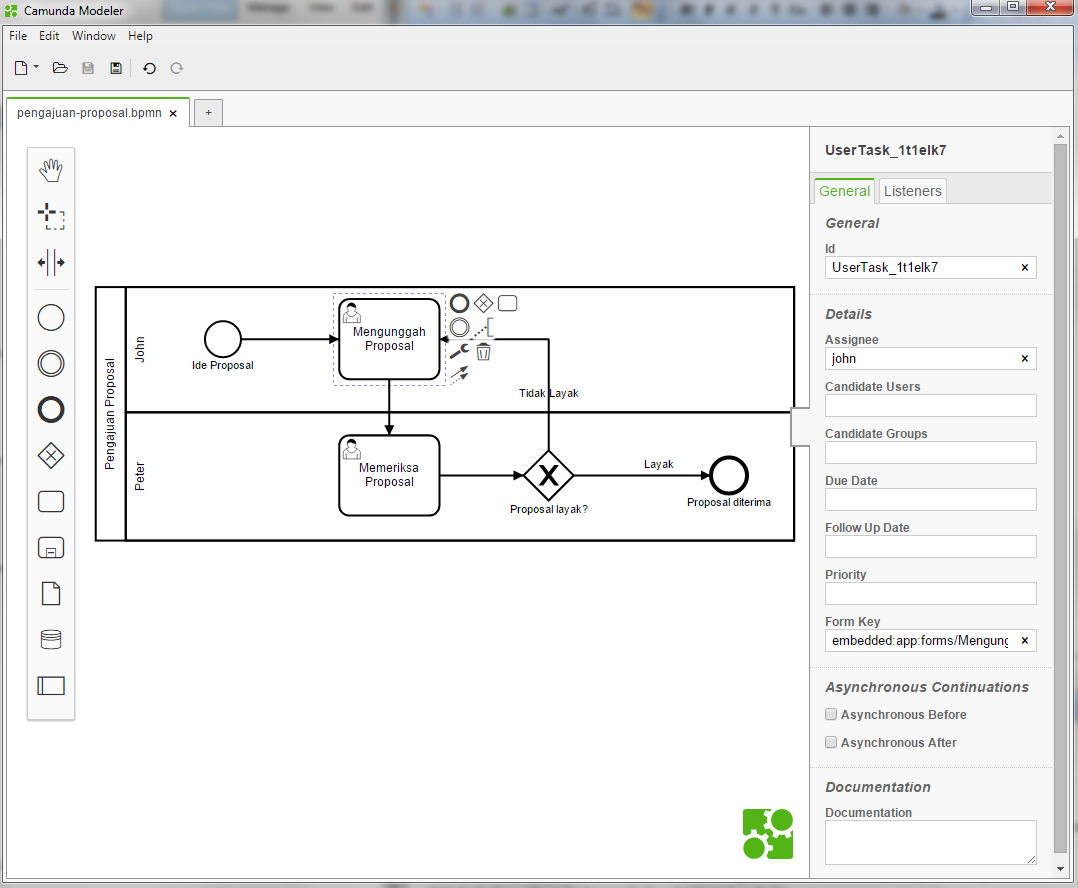
\includegraphics[scale=0.5]{Gambar/Bab-3/Kasus1-2}
			%\caption{Mengunggah Proposal} 
			%\label{fig:mengunggahproposal}
		%\end{figure}
		%
%Pada Gambar ~\ref{fig:mengunggahproposal}, terdapat beberapa atribut yang memiliki nilai, yaitu :
%\begin{itemize}
	%\item Id, yaitu id dari \textit{task} yang dipilih
	%\item Assignee, yaitu aktor yang akan mengerjakan \textit{task}
	%\item Form Key, yaitu tautan ke file HTML yang berupa tampilan untuk mengunggah proposal.
%\end{itemize}
\subsection{Modeler}
\label{modeler}
Camunda Modeler merupakan \textit{tool} untuk membuat diagram BPMN. \textit{File} yang dihasilkan dari \textit{tool} ini dapat dieksekusi menggunakan BPMS Camunda. Berikut ini adalah tampilan utama dari Camunda Modeler :

		\begin{figure}[H]
			\centering
			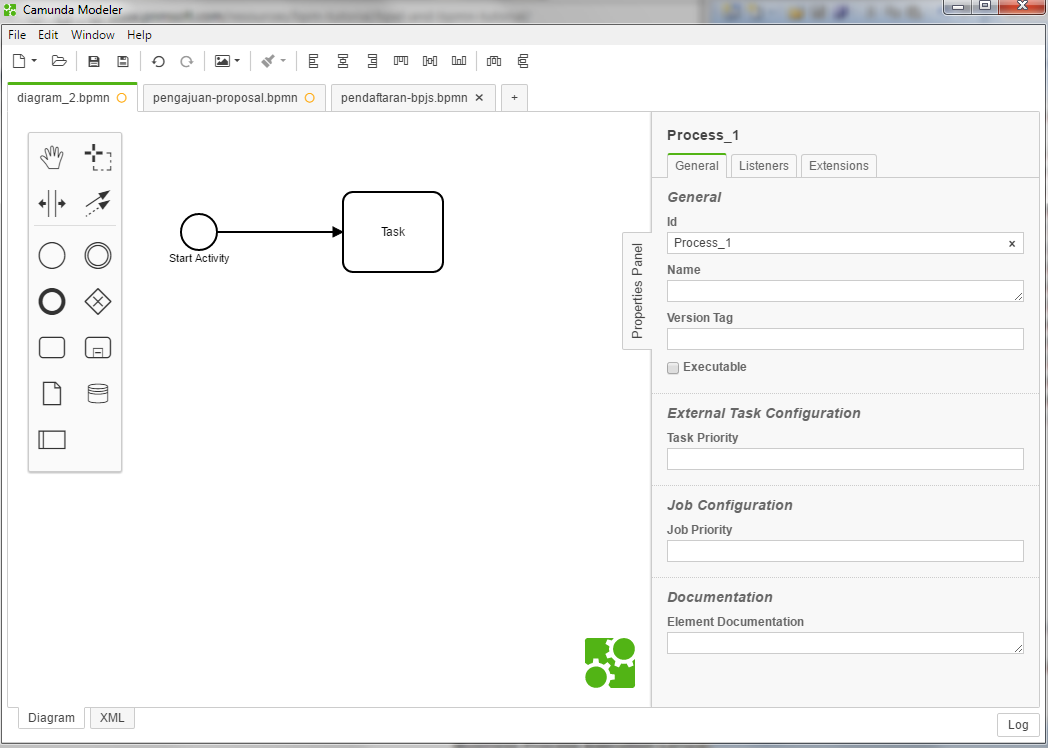
\includegraphics[scale=0.5]{Gambar/Bab-3/Modeler/1Awal}
			\caption{Tampilan Muka Camunda Modeler} 
			\label{fig:camundaModelerAwal}
		\end{figure}
		
Terdapat tiga bagian utama pada Camunda Modeler, yaitu :
\begin{enumerate}
	\item Bagian kiri merupakan kumpulan \textit{tool} dan notasi untuk membuat diagram BPMN.
	%\begin{figure}[H]
		%	\centering
			%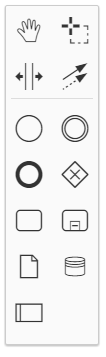
\includegraphics[scale=0.75]{Gambar/Bab-3/Modeler/2Notasi}
			%\caption{Tampilan Tools Camunda Modeler} 
			%\label{fig:camundaModelerTools}
		%\end{figure}
	\item Bagian kanan merupakan pengaturan untuk tiap \textit{event}, \textit{task}, maupun notasi lainnya. 
	%\begin{figure}[H]
		%\centering
		%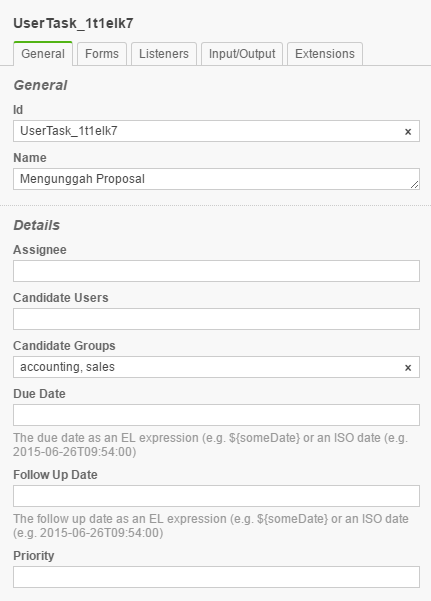
\includegraphics[scale=0.75]{Gambar/Bab-3/Modeler/3Properties}
		%\caption{Tampilan Pengaturan Camunda Modeler} 
		%\label{fig:camundaModelerProperties}
	%\end{figure}
	\item Bagian tengah merupakan tempat membuat diagram BPMN.
\end{enumerate}		


\subsection{Masalah Proses Bisnis}
\label{masalah}
Berikut ini berbagai masalah proses bisnis yang akan dimodelkan pada \textit{workflow} :

\subsubsection{Pengajuan Proposal}
Pegawai di perusahaan X memiliki tiga divisi yaitu \textit{accounting}, \textit{sales}, dan \textit{management}. Divisi \textit{accounting} dan \textit{sales} dapat mengajukan proposal bisnis ke divisi \textit{management}. Divisi \textit{management} harus memeriksa apakah proposalnya layak atau tidak. Jika proposalnya tidak layak, pembuat proposal harus memperbaiki dan mengunggahnya kembali. Workflow dari skenario ini sebagai berikut :

		\begin{figure}[H]
			\centering
			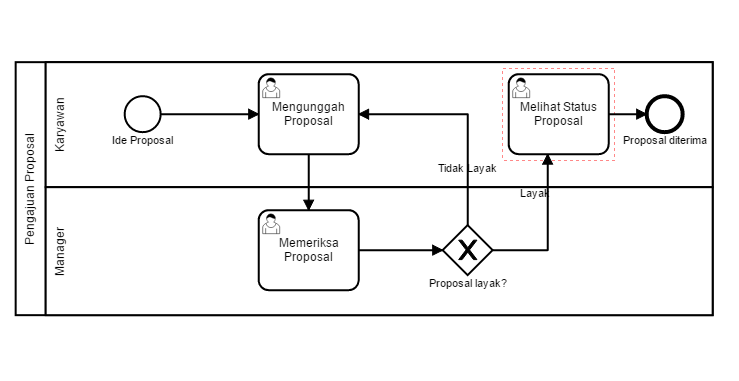
\includegraphics[scale=0.5]{Gambar/Bab-3/Kasus2-3}
			\caption{Mengunggah Proposal} 
			\label{fig:mengunggahproposalgroup}
		\end{figure}
%Pada Gambar ~\ref{fig:mengunggahproposalgroup}, terdapat atribut \textit{Candidate Groups}. Atribut ini melambangkan bahwa \textit{task} ini dapat dikerjakan oleh salah satu anggota dari grup \textit{accounting} atau grup \textit{sales}.

\subsubsection{Proses Pendaftaran BPJS}
\begin{enumerate}
	\item Pemohon mengisi formulir pendaftaran BPJS di situs BPJS (termasuk jenis keanggotaan).
	\item Pemohon mengupload semua dokumen persyaratan di situs BPJS.
	\item Sistem BPJS membangkitkan nomor pembayaran uang pendaftaran/ iuran pertama (nomor pembayaran selanjutnya menjadi nomor keanggotaan/ kartu BPJS).
  \item Pemohon melihat nomor pembayaran dan besarnya uang pendaftaran/ iuran pertama.
  \item Pemohon membayar uang pendaftaran/ iuran pertama melalui bank sesuai nomor pembayaran (paling lambat 3 hari setelah pendaftaran, jika lebih maka pendaftaran hangus).
  \item Pemohon memilih jadwal verifikasi dokumen asli yang tersedia.
  \item Sistem BPJS membangkitkan jadwal kedatangan dan nomor antrian.
  \item Pemohon mencetak jadwal kedatangan dan nomor antriannya.
  \item Pemohon datang ke kantor BPJS membawa dokumen asli (sesuai jadwal, jika tidak maka pendaftaran hangus). 
  \item Petugas BPJS memverifikasi pendaftaran, dan attachment dokumen persyaratan dan keasliannya. Jika valid dan lengkap, proses dilanjutkan ke langkah 11, jika tidak lengkap maupun tidak valid, maka kembali ke langkah 1.
	\item Sistem BPJS membangkitkan barcode untuk kartu BPJS.
  \item Petugas BPJS mencetak kartu BPJS dan meyerahkannya ke Pemohon.
\end{enumerate}
Workflow dari proses bisnis ini adalah sebagai berikut :
		
		\begin{figure}[H]
			\centering
			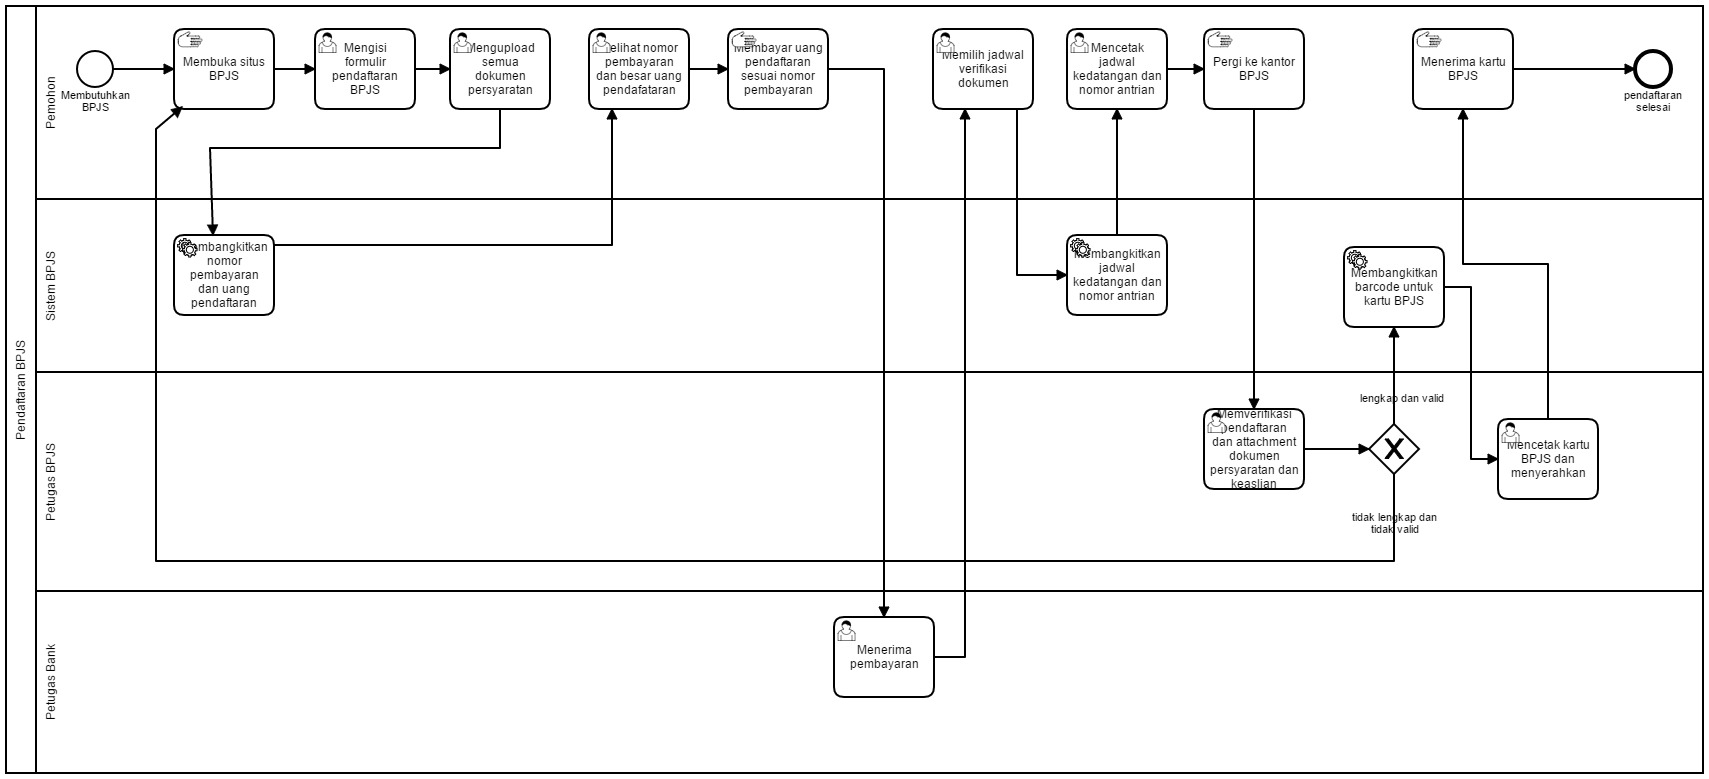
\includegraphics[scale=0.5]{Gambar/Bab-3/Kasus2-4}
			\caption{Pendaftaran BPJS} 
			\label{fig:mengunggahproposalgroup}
		\end{figure}






\section{BPMS Camunda}
\subsection{Instalasi Camunda}
\label{instalasicamunda}
Untuk menjalankan Camunda, diperlukan beberapa \textit{tool}\cite{bpmngetstarted:15:camunda}, yaitu :
\begin{itemize}
	\item Java JDK 1.7+.
	\item Apache Maven atau Maven yang sudah terpasang di Eclipse.
	\item Web browser.
	\item Camunda BPM Platform 
	\item Camunda Modeler
\end{itemize}


\subsubsection{Mempersiapkan Proyek Java}
\label{proyekjava}
\begin{description}
	\item Membuat Proyek Maven di Eclipse. 
		\begin{enumerate}
			\item Pilih File / New / Other / Maven / Maven Project kemudian pilih \textit{Next}.
			\item Pilih Create a simple project (skip archetype selection) kemudian pilih \textit{next}.
			\item Pilih Packaging : war, kemudian pilih Finish.
		\end{enumerate}
	\item Tambahkan \textit{Camunda Maven Dependencies} ke file pom.xml (lihat Lampiran ~\ref{lamp:pom}).
	\item Tambahkan sebuah kelas Process Application. Nama kelas dapat diganti dengan nama proses yang dibuat. 
	\begin{lstlisting}[language=java,basicstyle=\tiny,caption=Kelas Process Application]
	package org.camunda.bpm.getstarted.loanapproval;

import org.camunda.bpm.application.ProcessApplication;
import org.camunda.bpm.application.impl.ServletProcessApplication;

@ProcessApplication("Loan Approval App")
public class LoanApprovalApplication extends ServletProcessApplication {
  // empty implementation
}
	\end{lstlisting}
	\item Tambahkan \textit{Deployment Descriptor} di META-INF/processes.xml.
	
	\begin{lstlisting}[language=xml,basicstyle=\tiny,caption=processes.xml]	
	<?xml version="1.0" encoding="UTF-8" ?>

<process-application
    xmlns="http://www.camunda.org/schema/1.0/ProcessApplication"
    xmlns:xsi="http://www.w3.org/2001/XMLSchema-instance">

  <process-archive name="loan-approval">
    <process-engine>default</process-engine>
    <properties>
      <property name="isDeleteUponUndeploy">false</property>
      <property name="isScanForProcessDefinitions">true</property>
    </properties>
  </process-archive>

</process-application>
	\end{lstlisting}
	
\end{description}

\subsection{Menghubungkan BPMN dan BPMS Camunda}
\label{hubungkanbpmnbpms}
Untuk menhubungkan BPMN dan BPMS Camunda, akan digunakan kedua contoh kasus yang telah dibahas sebelumnya. 

\subsubsection{Kasus 1 : Pengajuan Proposal}
	
	\begin{figure}[H]
			\centering
			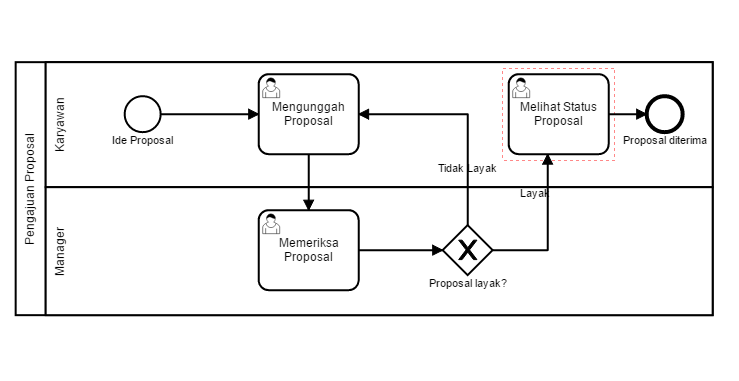
\includegraphics[scale=0.5]{Gambar/Bab-3/Kasus2-3}
			\caption{Mengunggah Proposal} 
			\label{fig:mengunggahproposalgroup}
		\end{figure}
		
		



\subsubsection{Memodelkan Proses}

	\begin{enumerate}
		\item Membuat file BPMN baru dengan File / New File / BPMN Diagram.
		\item Memodelkan proses.
				\begin{figure}[H]
			\centering
			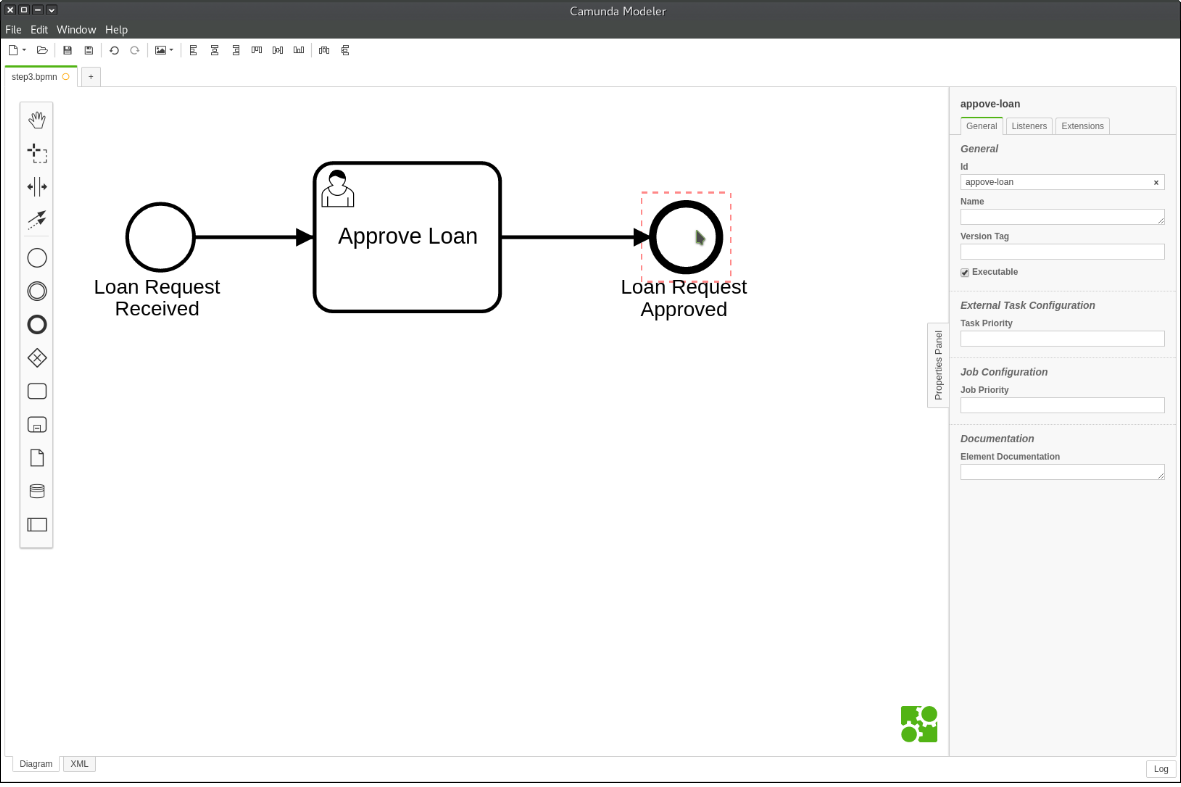
\includegraphics[scale=0.5]{Gambar/Bab-2/bpmn/bpmn}
			\caption{Contoh Model Proses} 
			\label{fig:modelproses}
		\end{figure}
		\item Menambahkan Form HTML pada User Task.
		\begin{lstlisting}[language=html,basicstyle=\tiny,caption=Contoh Task Form]
		<form name="approveLoan">
  <div class="form-group">
    <label for="customerId">Customer ID</label>
    <input class="form-control"
           cam-variable-type="String"
           cam-variable-name="customerId"
           name="customerId"
           readonly="true" />
  </div>
  <div class="form-group">
    <label for="amount">Amount</label>
    <input class="form-control"
           cam-variable-type="Double"
           cam-variable-name="amount"
           name ="amount" />
  </div>
</form>
\end{lstlisting}
		\item Menambahkan Service Task.
		\begin{lstlisting}[language=html,basicstyle=\tiny,caption=Contoh Implementasi Service Task]
		package org.camunda.bpm.getstarted.loanapproval;

import java.util.logging.Logger;
import org.camunda.bpm.engine.delegate.DelegateExecution;
import org.camunda.bpm.engine.delegate.JavaDelegate;

public class ProcessRequestDelegate implements JavaDelegate {

  private final static Logger LOGGER = Logger.getLogger("LOAN-REQUESTS");

  public void execute(DelegateExecution execution) throws Exception {
    LOGGER.info("Processing request by '"+execution.getVariable("customerId")+"'...");
  }

}
		\end{lstlisting}
	\end{enumerate}
	

\subsubsection{Menjalankan Camunda}
\label{menjalankancamunda}
	\begin{enumerate}
		\item Klik kanan pom.xml dan pilih Run As / Maven Install. Langkah ini akan menghasilkan file WAR di folder target.
		\item \textit{Copy paste} file WAR ke CAMUNDA\_HOME / server / apache-tomcat / webapps folder.
		\item Jalankan start-camunda.bat
	\end{enumerate}